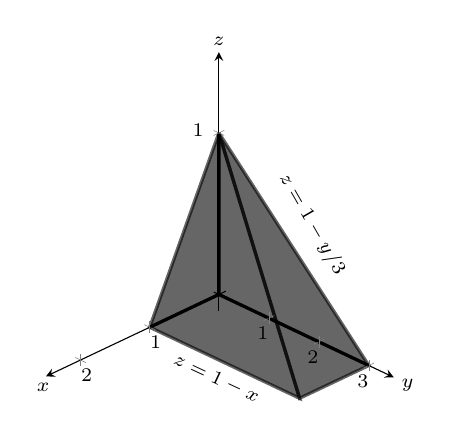
\begin{tikzpicture}[>=stealth]
\begin{axis}%
[width=175pt,height=200pt,
tick label style={font=\scriptsize},axis on top,
			axis lines=center,
			view={135}{25},
			name=myplot,
			xtick={1,2},
			ytick={1,2,3,4},
			ztick={1},
			%extra x ticks={1},
			%minor x tick num=1,
			%minor y tick num=4,
			%minor z tick num=1,
			%extra x tick labels={$a$},
			%extra y ticks={1},
			%extra y tick labels={$a$},
			%extra z ticks={1},
			%extra z tick labels={$h$},
			ymin=-.1,ymax=3.5,
			xmin=-.1,xmax=2.5,
			zmin=-.1, zmax=1.5,
			every axis x label/.style={at={(axis cs:\pgfkeysvalueof{/pgfplots/xmax},0,0)},xshift=-1pt,yshift=-4pt},
				xlabel={\scriptsize $x$},
			every axis y label/.style={at={(axis cs:0,\pgfkeysvalueof{/pgfplots/ymax},0)},xshift=5pt,yshift=-3pt},
				ylabel={\scriptsize $y$},
				every axis z label/.style={at={(axis cs:0,0,\pgfkeysvalueof{/pgfplots/zmax})},xshift=0pt,yshift=4pt},
				zlabel={\scriptsize $z$}
			]



%\addplot3[domain=0:1,y domain=0:1,%surf, %fill=white,
%%colormap={mp2}{\colormaptwo},opacity=.6,faceted color=black!40,
%samples=17,%samples y=10, very thin
%{\colortwo},very thick,samples y=0,smooth,] ({x},{4-x^2},{0});

\draw [very thick, {\colorone}] (axis cs:0,0,1) -- (axis cs:0,0,0) -- (axis cs:1,0,0)
																(axis cs: 0,0,0) -- (axis cs:0,3,0);
																
\draw [very thick, draw={\colorone},fill={\coloronefill},opacity=.6] (axis cs: 0,0,1) -- (axis cs: 1,0,0) -- (axis cs: 1,3,0) -- (axis cs:0,0,1);

\draw [very thick, draw={\colorone},fill={\colortwofill},opacity=.6] (axis cs: 0,0,1) -- (axis cs: 0,3,0) -- (axis cs: 1,3,0) -- (axis cs:0,0,1);



\draw  (axis cs: 1.3,1.75,0) node [rotate=-25] {\scriptsize $z=1-x$};% -- (axis cs: 1,0,.5);

\draw  (axis cs: .1,2,.75) node [rotate=-60] {\scriptsize $z=1-y/3$};

\end{axis}


\end{tikzpicture}












